\documentclass[12pt]{article}
\usepackage[a4paper, left=0.5cm, right=0.5cm, top=1cm, bottom=1cm]{geometry}
\usepackage{graphicx}
\usepackage{array}
\usepackage{booktabs}
\usepackage{keyval}
\graphicspath{{../images/}{./images}}
\usepackage{graphicx}
\usepackage{tikz}
\usepackage{xcolor}

\begin{document}
	\section*{\centering 1. Types of Plants}
	Identify and name the types of plants shown in the given images.\\[0.5cm]
	
	\begin{tabular}{@{}p{0.4cm}l@{}}
		\parbox[c][5.5cm][c]{0.4cm}{\rotatebox{90}{\textbf{Plants and its types}}} &
		\begin{tabular}{|m{4cm}|m{4cm}|m{4cm}|m{4cm}|}
			\hline
			\textbf{Images} & \textbf{Type of plant} & \textbf{Characteristics} & \textbf{Other plants with the same characteristics} \\ \hline
			
			\begin{tabular}[c]{@{}c@{}}%
				\parbox[c][2.5cm][c]{\linewidth}{\centering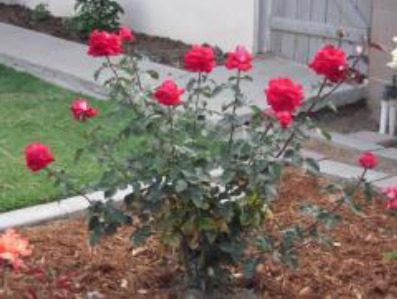
\includegraphics[width=2.5cm]{rose.jpg}}%
			\end{tabular} & Rose plant- & & \\ \hline
			
			\begin{tabular}[c]{@{}c@{}}%
				\parbox[c][2.5cm][c]{\linewidth}{\centering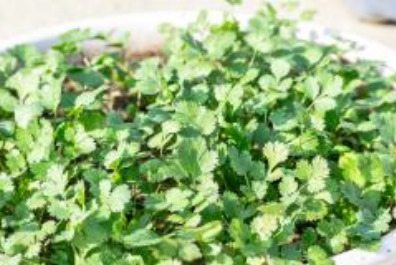
\includegraphics[width=2.5cm]{coriander.jpg}}%
			\end{tabular} & Coriander- & & \\ \hline
			
			\begin{tabular}[c]{@{}c@{}}%
				\parbox[c][2.5cm][c]{\linewidth}{\centering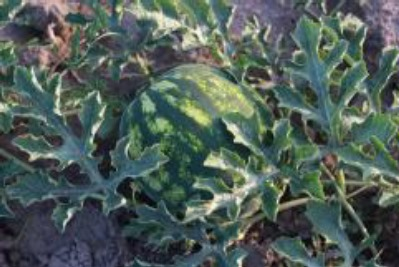
\includegraphics[width=2.5cm]{watermelon.jpg}}%
			\end{tabular} & Watermelon plant- & &\\ \hline
		\end{tabular}
	\end{tabular}\\[0.5cm]
	
	\textcolor{red}{\dotfill}
\end{document}
